\chapter{Finite Element Neutron Diffusion}
\label{ch:neutronDiffusion}

\section{Introduction}
  For typical nuclear reactor physics applications, diffusion theory
  approximates the neutron distribution within the reactor well. The neutron 
  diffusion equation is a second order partial differential equation in space.
  The neutron flux as the solution to the diffusion equation is continuous in
  both space and energy. In standard notation, the continuous neutron diffusion
  equation is presented as
  \begin{multline}\label{eq:continuous_diffusion}
    -\grad \cdot (D(\vr,E) \grad \varphi(\vr,E)) + \Sigma_t(\vr,E) 
      \varphi(\vr,E) = \\
      \frac{\chi(\vr,E)}{\keff} \int_0^{\infty} \nu_f(\vr,E') \Sigma_f(\vr,E') 
      \varphi(\vr,E') \; dE' + \int_0^{\infty} \Sigma_s(\vr,E' \rightarrow E) 
      \varphi(\vr,E') \; dE'
  \end{multline}
  Where $D$ is the diffusion constant, $\varphi$ is the continuous scalar 
  neutron flux, $\Sigma_t$ is the total cross section, $\chi$ is the effective 
  fission neutron spectrum, $\keff$ is the effective neutron multiplication 
  factor, $\Sigma_f$ is the fission cross section, $\nu_f$ is the neutron yield 
  per fission, and $\Sigma_s(\vr,E' \rightarrow E)$ is the scattering cross 
  section for neutrons at position $\vr$ scattering from energy $E'$ to $E$.
  
  The neutron diffusion equation must be discretized in space and 
  energy to be solved numerically. Energy discretization is relatively 
  straight-forward and is performed using the multigroup method. Spatial 
  discretization requires more attention and will be done with the Finite 
  Element Method (FEM). This spatial discretization method is selected for 
  several reasons. It allows for easily increasing the spatial convergence order
  of the method by increasing the order of the elements without refining the
  mesh. For example, for the same mesh, quadratic elements instead of linear
  elements could be used to improve the solution. Coordinates of nodes and 
  elements can be easily updated to reflect physical phenomena, such as thermal 
  expansion (\chref{ch:thermalExpansion}). Additionally, material properties are 
  calculated on an element basis allowing for fine detail updates to the 
  material properties during the calculation in future applications.
  
  For energy discretization with the multigroup method, an energy structure is 
  described as $\{E_g\}$ for $g = 0,1,2,\ldots,G$ and by in order of decreasing 
  energy by convention.
  \[ 0 < E_G < E_{G-1} < \ldots < E_2 < E_1 < E_0 \]
  Then, multigroup constants can be calculated based on the energy group 
  structure and the known cross sections. Multigroup constants are calculated to
  preserve the number of neutrons produced or destroyed. That is, the 
  calculation preserves reaction rates where the reaction rate for reaction $x$
  is defined as $R_x=\Sigma_x \varphi$. A formal derivation is given in 
  \cite{duderstathamilton} and the results are presented below.
  \begin{align}
    D_g(\vr) &= \frac{\int_{E_g}^{E_{g-1}} D(\vr,E') \grad \varphi(\vr,E)\;dE}
      {\int_{E_g}^{E_{g-1}} \grad \varphi(\vr,E)\;dE} \\
    \Sigma_{t,g}(\vr) &= \frac{\int_{E_g}^{E_{g-1}} \Sigma_t(\vr,E) 
      \varphi(\vr,E)\;dE}{\int_{E_g}^{E_{g-1}} \varphi(\vr,E)\;dE} \\
    \nu\Sigma_{f,g}(\vr) &= \frac{\int_{E_g}^{E_{g-1}} \nu_f(\vr,E)
      \Sigma_f(\vr,E) \varphi(\vr,E)\;dE}{\int_{E_g}^{E_{g-1}} 
      \varphi(\vr,E)\;dE} \\
    \Sigma_{s,g\rightarrow g'}(\vr) &= \frac{\int_{E_g'}^{E_{g'-1}} 
      \int_{E_g}^{E_{g-1}} \Sigma_s(\vr,E' \rightarrow E) 
      \varphi(\vr,E')\;dE\;dE'}
      {\int_{E_g}^{E_{g-1}} \varphi(\vr,E)\;dE}  \\
    \chi_g(\vr) &= \int_{E_g}^{E_{g-1}} \chi(\vr,E) \; dE \\
    \phi_g(\vr) &= \int_{E_g}^{E_{g-1}} \varphi(\vr,E) \; dE
  \end{align}
  Note that cross sections $\nu_f(\vr,E)$ and $\Sigma_f(\vr,E)$ have been 
  combined. This is a convenient mathematical representation of the group
  collapse to preserve the rate of neutrons produced. This is not, however, how
  multigroup constants are actually calculated. The derivation assumes that
  material cross sections and flux distributions are known continuously with
  respect to energy. This is never the case as material cross sections are
  measured from experiments and flux distributions are only known continuously
  for select problems. More typically, these multigroup constants are measured
  experimentally for a many group structure and then a group collapse is
  performed discretely. For the purposes of this application, it is sufficient
  to assume that the constants are provided from some higher order flux
  calculation method.

  \eref{eq:continuous_diffusion} can be discretized in energy as
  \begin{align}\label{eq:multigroup_diffusion}
    - \grad \cdot ( D_g(\vr) \grad \phi_g(\vr)) + \Sigma_{t,g}(\vr) \phi_g(\vr)= 
      \frac{\chi_g(\vr)}{\keff} \sum_{g'=1}^{G} \nu\Sigma_{f,g'}(\vr) 
      \phi_{g'}(\vr) + \sum_{g'=1}^{G} \Sigma_{s,g' \rightarrow g}(\vr) 
      \phi_{g'}(\vr)
  \end{align}
  The neutron diffusion equation has now been discretized in energy.
  Spatial dicretization will be based on the Finite Element Method (FEM) and 
  will be discussed in \sref{sec:formulation:derivation}.
  
  The total neutron cross section includes the contribution due to 
  self-scattering. That is, due to $\Sigma_{s,g\rightarrow g}$. This can be 
  removed from \eref{eq:multigroup_diffusion} for simplicity and numeric
  efficiency.
  \begin{equation} \label{eq:multigroup_removal}
    - \grad \cdot( D_g(\vr) \grad \phi_g(\vr)) + \Sigma_{r,g}(\vr) \phi_g(\vr) = 
      \frac{\chi_g(\vr)}{\keff} \sum_{g'=1}^{G} \nu\Sigma_{f,g'}(\vr) 
      \phi_{g'}(\vr) + \sum_{g'=1, g' \ne g}^{G} 
      \Sigma_{s,g' \rightarrow g}(\vr) \phi_{g'}(\vr)
  \end{equation}
  Where $\Sigma_{r,g}$ is the removal cross section defined as 
  $\Sigma_{r,g}(\vr) = \Sigma_{t,g}(\vr) - \Sigma_{s,g\rightarrow g}(\vr)$. For
  simplicity, the neutron sources in \eref{eq:multigroup_removal} can be 
  combined into a single term.
  \begin{equation} \label{eq:multigroup_source}
    - \grad \cdot( D_g(\vr) \grad \phi_g(\vr)) + \Sigma_{r,g}(\vr) \phi_g(\vr) = 
      q_g(\vr)
  \end{equation}
  Where $q_g(\vr)$ is the combined neutron source at position $\vr$ for energy 
  group $g$. The combined source form is useful for solving the
  multigroup neutron diffusion problem for an arbitrary number of groups.
  \eref{eq:multigroup_source}
  is solved for each energy group and interaction between groups is
  described in the source term, $q_g(\vr)$. In other literature, the multigroup
  equation may be
  solved for each group simultaneously by treating interaction between groups
  explicitly. By solving each group independently (as done here) the method 
  remains general. Additionally, for many-group energy structures, as common to
  fast reactor applications, solving each group independently is typically more
  computationally efficient as linear systems have favorable conditioning and
  remain smaller.
  
  It is sometimes desirable to partition $q$ into contributions due 
  to fission ($q_{fiss}$), up-scattering ($q_{up}$) when a neutron increases in 
  energy, and down-scattering when a neutron decreases in energy ($q_{down}$).
  \begin{align}
    q_g(\vr) &= q_{fiss,g}(\vr) + q_{up,g}(\vr) + q_{down,g}(\vr) \\
    \label{eq:qfiss}
    q_{fiss,g}(\vr) &= \frac{\chi_g(\vr)}{\keff} \sum_{g'=1}^{G} 
      \nu \Sigma_{f,g'}(\vr) \phi_{g'}(\vr) \\
    \label{eq:qup}
    q_{up,g}(\vr) &= \sum_{g'=g+1}^{G} \Sigma_{s,g' \rightarrow g}(\vr)
      \phi_{g'}(\vr) \\
    \label{eq:qdown}
    q_{down,g}(\vr) &= \sum_{g'=1}^{g-1} \Sigma_{s,g' \rightarrow g}(\vr)
      \phi_{g'}(\vr)
  \end{align}
  Where the difference between $q_{up}$ and $q_{down}$ are the limits of the 
  summation. This form allows for operator splitting of the neutron source term.
  In an iterative scheme, it will be necessary for fission and up-scatter 
  sources to use a different flux iterate than down-scatter so this division
  will prove useful.

\section{Formulation of Finite Element Equations}
  \subsection{Derivation}
    \label{sec:formulation:derivation}
    The only remaining continuous variable in the problem to be discretized is 
    the spatial variable $\vr$. This will be discretized according to the Finite 
    Element  Method (FEM). The problem is solved in a finite domain 
    $\vr \in \Omega$ where $\partial \Omega$ represents the boundary of the 
    domain where some boundary condition is specified. Boundary condition 
    options provided include
    \begin{enumerate}
      \item Mirror. $\grad \phi_g(\vr) = 0$ for $\vr \in \partial \Omega$.
      \item Albedo. $D_g(\vr) \grad \phi_g(\vr) + \albedo \phi_g(\vr)=0$ for 
        $\vr \in \partial \Omega$ where $\albedo$ is a real constant specified
        by the user. For vacuum conditions, $\albedo = \half$.
      \item Zero Flux. $\phi_g(\vr) = 0$ for $\vr \in \partial \Omega$.
    \end{enumerate}
    (Note: the order of the above list corresponds to the order of boundary 
    condition precedent in code with the greater the integer, the greater the 
    precedent.)
    
    FEM begins by dividing the spatial domain $\Omega$
    into a set of elements.
    \[ \Omega = \Omega_1 \cup \Omega_2 \cup \Omega_3 \cup \ldots \cup
      \Omega_{N_E} \]
    where $\{\Omega_e\}$ for $e = 1,2,\ldots,N_E$ is a set of
    nonoverlapping elements and $N_E$ is the number of elements in the problem.
    Elements are in an unstructured grid and can be generated by any method to
    describe the geometry of the problem.
    
    Finite element derivation begins with \eref{eq:multigroup_source}.
    The equation is multiplied by a testing function $v(\vr) \in H_1(\Omega)$ 
    Where $H$ is the Sobolev Space. 
    \begin{equation}
      -\grad \cdot (D_g(\vr) \grad \phi_g(\vr)) v(\vr) + 
        \Sigma_{r,g}(\vr) \phi_g(\vr) v(\vr) =
        q_g(\vr) v(\vr)
    \end{equation}
    Then, the equation is integrated over the problem domain. This integration
    yields the Weak Form or Variational Form of the problem.
    \begin{equation}
      - \int_{\Omega} \grad \cdot (D_g(\vr) \grad \phi_g(\vr)) v(\vr) \; d\Omega
        \int_{\Omega} \Sigma_{r,g}(\vr) \phi_g(\vr) v(\vr) \;d\Omega =
        \int_{\Omega} q_g(\vr) v(\vr) \;d\Omega
    \end{equation}
    
    For the purposes of this application, material cross sections and the
    neutron source are assumed to be constant within an element. Then, the 
    integral can be partitioned into a sum of integrals over the elements in the
    domain assuming the set of elements 
    \begin{equation} \label{eq:element_by_element}
      -\sum_{e=1}^{N_E} D_{g,e} 
        \int_{\Omega_e} \grad \cdot \grad \phi_g(\vr) v(\vr) \; d\Omega_e +
        \sum_{e=1}^{N_E} \Sigma_{r,g,e} \int_{\Omega_e} \phi_g(\vr) v(\vr) 
        \;d\Omega_e = \sum_{e=1}^{N_E} q_{g,e} \int_{\Omega_e} v(\vr) 
        \; d\Omega_e
    \end{equation}
    The Second Green's Theorem is used to simplify the integral in the first
    term. A proof can be found in \cite{textbookli} in Theorem 9.2. The Second 
    Green's Theorem is in \eref{eq:greens}.
    \begin{equation} \label{eq:greens}
      -\int_{\Omega_e} \grad \cdot \grad \phi_g(\vr) v(\vr) \;d\Omega_e =
        -\int_{\partial \Omega_e}  
        \frac{\partial \phi_g(\vr)}{\partial \vn} v(\vr)\; ds + \int_{\Omega_e} 
        \grad \phi_g(\vr) \cdot \grad v(\vr) \; d\Omega_e
    \end{equation}
    Where $\frac{\partial \phi_g(\vr)}{\partial \vn}$ is the outward normal 
    derivative, sometimes written $\grad_{\vn} \phi_g(\vr)$, and the integral 
    $ds$ is a line integral in two dimensions or a surface integral in three 
    dimensions. Recognizing that this quantity will only be relevant on the 
    boundary of the problem, the value of the outward normal derivative may be 
    specified in a boundary condition. Specifically, the albedo boundary 
    condition which has the following form for $\vr \in \partial \Omega$. 
    \begin{align}
      D_g(\vr) \grad \phi_g(\vr) + \albedo \phi_g(\vr) &= 0 \\
      D_g(\vr) \grad \phi_g(\vr) &= -\albedo \phi_g(\vr)
    \end{align}
    Substituting \eref{eq:greens} into  \eref{eq:element_by_element} and 
    assuming the outward normal derivative is specified in the form of an albedo
    boundary condition.
    \begin{multline} 
      -\sum_{e=1}^{N_E} D_{g,e} \int_{\partial \Omega_e} v(\vr) 
        \frac{\partial \phi_g(\vr)}{\partial \vn} \;ds + \sum_{e=1}^{N_E} D_{g,e}
        \int_{\Omega_e} \grad \phi_g(\vr) \cdot \grad v(\vr) \; d\Omega_e + \\
        \sum_{e=1}^{N_E} \Sigma_{r,g,e} \int_{\Omega_e} \phi_g(\vr) v(\vr) 
        \; d\Omega_e =
        \sum_{e=1}^{N_E} q_{g,e} \int_{\Omega_e} v(\vr) \; d\Omega_e
    \end{multline}
    \begin{multline} \label{eq:element_boundary}
      \sum_{e=1}^{N_E} \albedo \int_{\partial \Omega_e} v(\vr) 
        \phi_g(\vr) \;ds + \sum_{e=1}^{N_E} D_{g,e}
        \int_{\Omega_e} \grad \phi_g(\vr) \cdot \grad v(\vr) \; d\Omega_e + \\
        \sum_{e=1}^{N_E} \Sigma_{r,g,e} \int_{\Omega_e} \phi_g(\vr) v(\vr) 
        \; d\Omega_e =
        \sum_{e=1}^{N_E} q_{g,e} \int_{\Omega_e} v(\vr) \; d\Omega_e
    \end{multline}
    Now the function of interest $\phi_g(\vr)$ is assumed to be a linear 
    combination of chosen basis functions $\{\basis_i\}$.
    \begin{equation} \label{eq:linear_combination}
      \phi_g(\vr) = \sum_{i=1}^{DOF} \beta_{g,i} \basis_i(\vr)
    \end{equation}
    Where coefficients $\{\beta_i\}$ are unknown and will be determined and $DOF$
    is the degree of freedom of the problem. Typically $DOF$ is the number of
    nodes minus any nodes for which the flux is fixed (e.g. zero-flux nodes).
    Typically, these basis functions have unit magnitude and are centered at the
    node  points so the coefficients $\beta_i$ are the approximated solution at
    the nodes. It is also convenient for basis functions to have compact
    support. That is, basis functions are created such that they are non-zero in
    only one element and zero in all other elements.
    Basis functions are typically piecewise continuous polynomials of arbitrary 
    degree. For selected elements, basis functions will be defined explicitly in
    \sref{sec:matrix_quantities}.
    Linear and quadratic polynomials are common but for the application 
    presented here, only linear basis functions are explored.
    The test function $v(\vr)$ is also chosen as a linear combination of the 
    basis functions.
    \begin{equation} \label{eq:linear_superposition}
      v(\vr) = \sum_{j=1}^{DOF} \basis_j(\vr)
    \end{equation}
    The testing function is arbitrary so the magnitude is fixed to the magnitude
    of the basis function.
    
    \eref{eq:linear_combination} and \eref{eq:linear_superposition} are inserted 
    into \eref{eq:element_boundary}.
    \begin{multline}
      \sum_{e=1}^{N_E} \albedo \sum_{i=1}^{N} \beta_{i,g}
        \int_{\partial \Omega_e}
        \basis_i(\vr)  \basis_j(\vr) \;ds +
        \sum_{e=1}^{N_E} D_{g,e} \sum_{i=1}^{N} \beta_{i,g}
        \int_{\Omega_e} \grad \basis_i(\vr) \cdot \grad \basis_i(\vr)\;d\Omega_e
        + \\
        \sum_{e=1}^{N_E} \Sigma_{r,g,e} \sum_{i=1}^{N} \beta_{i,g}
        \int_{\Omega_e} \basis_i(\vr) \basis_i(\vr) \; d\Omega_e =
        \sum_{e=1}^{N_E} q_{g,e} \sum_{i=1}^{N} 
        \int_{\Omega_e} \basis_i(\vr) \; d\Omega_e
    \end{multline}
    This can be rearranged as a linear system of equations.
    \begin{multline}
      \sum_{i=1}^{N} \beta_{i,g} \sum_{j=1}^{N} \left(
        \sum_{e=1}^{N_E} \albedo \int_{\partial \Omega_e}
        \basis_i(\vr)  \basis_j(\vr) \;ds +
        \sum_{e=1}^{N_E} D_{g,e} 
        \int_{\Omega_e} \grad \basis_i(\vr) \cdot \grad \basis_j(\vr)\;d\Omega_e
        \right.
        + \\
        \left.
        \sum_{e=1}^{N_E} \Sigma_{r,g,e}
        \int_{\Omega_e} \basis_i(\vr) \basis_j(\vr) \; d\Omega_e \right) =
        \sum_{i=1}^{N} \left(
        \sum_{e=1}^{N_E} q_{g,e} 
        \int_{\Omega_e} \basis_i(\vr) \; d\Omega_e \right)
    \end{multline}
    Which can be written in matrix format as
    \begin{equation}
      \label{eq:fem_notation}
      a(\basis_i,\basis_j) = f(\basis_i)
    \end{equation}
    Or in the notation common to the FEM
    \begin{equation}
      \label{eq:matrix_notation}
      \ma \vu = \vf
    \end{equation}
    $a(\basis_i,\basis_j)$ is the bilinear form and $f(\basis_i)$ is the linear 
    form of the finite element system. The notation of \eref{eq:fem_notation} is
    common to mathematical discussions of the FEM. The diffusion coefficient 
    $D_g(\vr)$ is non-zero and bounded and the removal cross section 
    $\Sigma_{r,g}(\vr)$ is bounded. The Lax-Milgram Lemma implies the solution
    to the FEM as derived here is both unique and bounded (See Theorem 9.3
    \cite{textbookli}). This is 
    not the entire description as the source function $q_g(\vr)$ is updated on 
    each power iteration. What the satisfaction of the Lax Milgram Lemma does 
    imply in this instance is that for a fixed source on a given problem 
    iteration, a unique solution exists. The global problem remains an 
    eigenvalue problem as described in \cite{duderstathamilton}. The power
    iteration method will 
    return the fundamental eigenvalue $\keff$ and the fundamental 
    eigenmode $\phi$ which may be normalized by an arbitrary constant.
    
    In matrix notation \eref{eq:matrix_notation}. Matrix $\ma$ is 
    described by integral quantities, vector $\vu$ is the unknown magnitudes of
    the basis functions $\{\beta_i\}$, and vector $\vf$ is described by the 
    source integral quantity. Inspecting the matrix $\ma$ and the vector $\vf$
    reveals the following.
    \begin{align}
      \label{eq:matrix_population}
      A_{i,j,g,e} &= \albedo \int_{\partial \Omega_e} \basis_i(\vr) 
        \basis_j(\vr) \; ds + D_{g,e} 
        \int_{\Omega_e} \grad \basis_i(\vr) \cdot \grad \basis_j(\vr) \;
        d\Omega_e + \Sigma_{r,g,e} \int_{\Omega_e} \basis_i(\vr) \basis_j(\vr)
        \; d\Omega_e \\
      \label{eq:vector_population}
      f_{i,g,e} &= q_{g,e} \int_{\Omega_e} \basis_i(\vr) \;d\Omega_e
    \end{align}
    Then, 
    \begin{align}
      A_{i,j,g} &= \sum_{e=1}^{N_E} A_{i,j,g,e} \\
      f_{i,g} &=  \sum_{e=1}^{N_E} f_{i,g,e}
    \end{align}
    which leads to the natural population of the matrix $\ma$ on an 
    element-by-element basis. That is, the matrix $\ma$ is assembled by looping
    through all of the elements and summing their contribution to the matrix. 
    Note that the contribution due to the surface integral will be zero in 
    elements not on the boundary and may also be zero for problems with select
    boundary conditions. See \sref{sec:boundary_conditions} for boundary
    condition discussion.  The population of the vector $\vf$ is done similarly. 
    Then, the matrix $\ma$ and the vector $\vf$ are known for each energy group.
    The equations are solved for one group at a time and $\phi_g$ is calculated
    and stored.
    
    Though the notation may be obtuse, the above reduces to a linear system of
    equations. These equations are constructed from the integral quantities 
    specified by the FEM and the coefficients given by the cross sections and
    fixed source regions. The integral quantities themselves are expressed 
    explicitly in the next section.
    
  \subsection{Matrix Quantities}
    \label{sec:matrix_quantities}
    For certain simple elements, the integral quantities described in 
    \eref{eq:matrix_population} and \eref{eq:vector_population} have exact 
    analytic forms. For this application, linear triangles and linear wedges
    are investigated and many of the integrals have exact expressions. If these 
    quantities cannot be expressed exactly or doing so would be computationally
    difficult, quadratures can be used and for certain problems, these 
    quadratures can express the integrals exactly. This will be discussed in 
    \sref{sec:quadratures}.
    \subsubsection{Linear Triangles}
      Linear triangles are common to two-dimensional finite element methods and
      have been investigated in many applications \cite{Hosseini2017} 
      \cite{Hosseini2013} \cite{Hosseini2015}. The linear triangle element is a
      triangle  defined by three corner coordinates with basis functions located 
      on each corner. A triangle element is sketched in 
      \fref{fig:sketch_triangle}.
      \begin{figure}
        \centering
        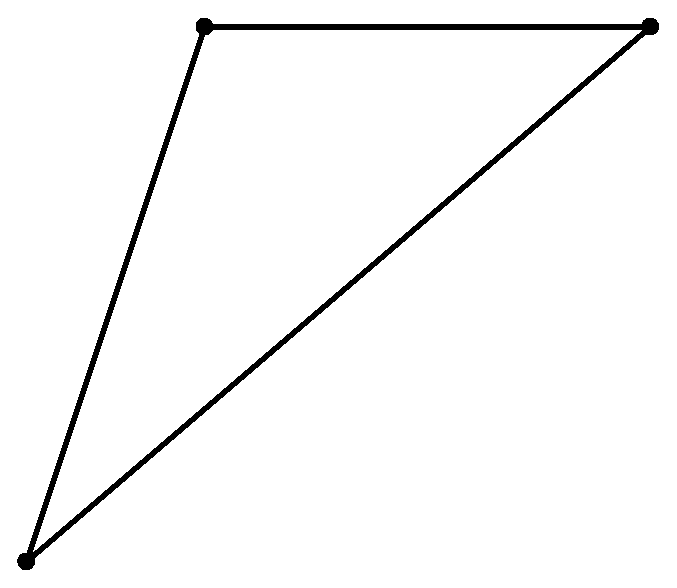
\includegraphics[width=0.3\textwidth]{sketch_triangle}
        \caption{Description of Triangle Element.}
        \label{fig:sketch_triangle}
      \end{figure}
      It is difficult to analytically calculate the desired integral quantities
      for an arbitrary triangle. Instead, a simplified reference element is
      created and quantities are calculated for the reference element and then
      translated to the arbitrary element using a Jacobian. 
      The reference triangle $T_{ref}$ is located in
      $\xi \in [0,1]$ and $\eta \in [0,1-\xi]$. The basis functions are zero
      outside of the reference triangle and within the reference triangle, 
      basis functions for the are provided.
      \begin{align}
        \basis_i(\xi,\eta) &= 0 \; \forall \; (\xi,\eta) \notin T_{ref} \\
        \basis_1(\xi,\eta) &= \xi \\
        \basis_2(\xi,\eta) &= \eta \\
        \basis_3(\xi,\eta) &= 1-\xi-\eta
      \end{align}
      
      There are simple expressions
      for the integral quantities for an arbitrary triangle that are originally
      proposed in \cite{textbookwhite}. The expression for
      the line integral is found in \cite{computerLab}. For a triangle with 
      corners $\{ x_i,y_i \}$ with $i=1,2,3$.
      \begin{align}
        \int_{\Omega_e} \grad \basis_i(\vr) \cdot \grad \basis_j(\vr) 
          \;d\Omega_e &= \frac{1}{4 A_e}
          ((x_{i+1}-x_{i+2})(x_{j+1}-x_{j+2}) + 
          (y_{i+1}-y_{i+2})(y_{j+1}-y_{j+2})) \\
        \int_{\Omega_e} \basis_i(\vr) \basis_j(\vr) \;d\Omega_e &= 
          \frac{A_e}{12} (1+\delta_{ij}) \\
        \int_{\Omega_e} \basis_i(\vr) \;d\Omega_e &= \frac{A_e}{3} \\
        \int_{\partial \Omega_e} \basis_i(\vr) \basis_j(\vr) \;ds &=
          \frac{L_e}{6}(1+\delta_{ij}) \\
      \end{align}
      Where $A_e$ is the area of the triangular element, $L_e$ is the length of 
      the edge between node $i$ and node $j$, and $\delta_{ij}$ is the Kronecker
      delta. The area of a triangle in three dimensions is calculated for a
      triangle with corners $\vc_i = (x_i, y_i, z_i)$ with $i=1,2,3$ where
      $\vc_i$ is a coordinate vector for notational simplicity.
      \begin{align}
        \va &= \vc_2 - \vc_1 \\
        \vb &= \vc_3 - \vc_1 \\
        A_e &= \half \lvert \va \times \vc \rvert \\
        &= \half \sqrt{ (a_2 b_3 - a_3 b_2)^2 + (a_3 b_1 - a_1 b_3)^2 +
          (a_1 b_2 - a_2 b_1)^2}
      \end{align}
      The Kronecker delta is defined as
      \begin{equation} \label{eq:kroneker_delta}
        \delta_{ij} =
        \begin{cases}
          0 & \text{if } i \ne j \\
          1 & \text{if } i = j
        \end{cases}
      \end{equation}
      For higher order triangular elements, it will be necessary to employ a 
      quadrature.
    \subsubsection{Linear Wedges}
      Wedge elements have not achieved the same commonality as triangular 
      elements but are, in their simplest form, extruded triangles. The general
      wedge, however, is more general than extrusion. In this application,
      wedges are useful to describe hexagonal geometries such as fast spectrum
      reactors. Reactor geometries are also typically described in lattices so
      the wedge element allows for easily ``stacking'' lattices on top of each
      other.

      Geometrically, the wedge element is a pentahedron with six corner nodes,
      sometimes referred to as a triangular prism. However,
      their exact geometric relation is not fixed and the nodes are free to 
      expand and distort. That is, each node is free to move independently of
      all other nodes. These shapes are unique because three of the faces are
      quadrilateral and two of the faces are triangular. A typical (left) and 
      distorted (right) wedge element is described in \fref{fig:sketch_wedge}.
      \begin{figure}
        \centering
        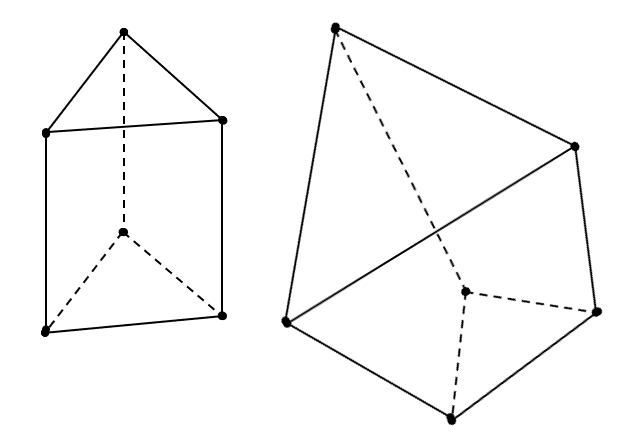
\includegraphics[width=0.6\textwidth]{sketch_wedge}
        \caption{Description of Typical and Distorted Wedge Elements.}
        \label{fig:sketch_wedge}
      \end{figure}
      The reference wedge $W_{ref}$ is located in 
      $\xi \in [0,1]$, $\eta \in [0,1-\xi]$, and $\zeta \in [-1,1]$. The basis
      functions are, again, zero outside of the reference wedge and are provided
      within the reference wedge.
      \begin{align}
        \basis_i(\xi,\eta,\zeta) &= 0 \; \forall \; (\xi,\eta,\zeta)
          \notin W_{ref} \\
        \basis_1(\xi,\eta,\zeta) &= \half (1-\zeta)(1-\xi-\eta) \\
        \basis_2(\xi,\eta,\zeta) &= \half (1-\zeta)\xi \\
        \basis_3(\xi,\eta,\zeta) &= \half (1-\zeta)\eta \\
        \basis_4(\xi,\eta,\zeta) &= \half (1+\zeta)(1-\xi-\eta) \\
        \basis_5(\xi,\eta,\zeta) &= \half (1+\zeta)\xi \\
        \basis_6(\xi,\eta,\zeta) &= \half (1+\zeta)\eta 
      \end{align}

      The values presented herein are not found in literature and are 
      calculated by the author.
      \begin{align}
        \label{eq:bigmat}
        \int_{\Omega_e} \basis_i(\vr) \basis_j(\vr) \;d\Omega_e &= 
          \frac{V_e}{2}
          \begin{pmatrix}
            \frac{1}{18} & \frac{1}{36} & \frac{1}{36} & \frac{1}{36} & 
              \frac{1}{72} & \frac{1}{72} \\
            \frac{1}{36} & \frac{1}{18} & \frac{1}{36} & \frac{1}{72} & 
              \frac{1}{36} & \frac{1}{72} \\
            \frac{1}{36} & \frac{1}{36} & \frac{1}{18} & \frac{1}{72} & 
              \frac{1}{72} & \frac{1}{36} \\
            \frac{1}{36} & \frac{1}{72} & \frac{1}{72} & \frac{1}{18} & 
              \frac{1}{36} & \frac{1}{36} \\
            \frac{1}{72} & \frac{1}{36} & \frac{1}{72} & \frac{1}{36} & 
              \frac{1}{18} & \frac{1}{36} \\
            \frac{1}{72} & \frac{1}{72} & \frac{1}{36} & \frac{1}{36} & 
              \frac{1}{36} & \frac{1}{18} 
          \end{pmatrix} \\
        \int_{\Omega_e} \basis_i(\vr) \;d\Omega_e &= \frac{V_e}{12} \\
        \int_{\partial \Omega_e} \basis_i(\vr) 
          \basis_j(\vr) \;d\partial\Omega_e &= 
          \begin{cases}
            \frac{A_{\Delta}}{12}(1+\delta_{ij}) & \text{if triangle} \\
            \frac{A_{\Box}}{36}(1+\delta_{ij})(1-\half \delta_{i,(5-j)}) &
              \text{if quadrilateral}
          \end{cases}
      \end{align}
      Where $V_e$ is the volume of the element. For a simple extruded triangle,
      the volume calculation is straightforward. However, allowing the nodes to
      move with respect to each other makes the volume of the element difficult
      to calculate. Instead, the Jacobian is used to calculate $V_e$. The
      relationship is given in \tref{tab:jacobi}. The element is isoparametric
      (has constant Jacobian determinant) for any point within the reference
      wedge, such as (0,0,0). Then $V_e = 2 \lvert \mj \rvert$.
      
      This matrix in \eref{eq:bigmat} is indexed $M_{ij}$
      and is presented as a matrix because of its irregular form. Notice the 
      integral containing the gradient operator has been omitted because if 
      it could be computed analytically, it would be less computationally 
      efficient than using a quadrature.
  \subsection{Quadratures}
    \label{sec:quadratures}
    Quadratures are sets of coordinates and weights which allow for the exact 
    integration of polynomials of given order. For a given set of weights 
    $\{w_i\}$ and a set of coordinates $\{\vx\}$, the quadrature can be 
    expressed as follows.
    \begin{equation}
      \label{eq:quadrature}
      \int_{\Omega} f(\vx) \;d\Omega \approx \sum_{i=1}^{N} w_i f(\vx_i)
    \end{equation}
    where $\Omega$ is an arbitrary domain described by $\{\vx_i\}$. The 
    quadratures in \eref{eq:quadrature} will exactly integrate a polynomial of
    the order of the quadrature. It is not necessarily true that $N$ be the 
    order of the quadrature.
    
    For one-dimensional integrals, the Gaussian quadrature is common and the 
    most compact quadrature. The Gaussian quadrature exactly integrates a 
    polynomial of order $n$ using exactly $n$ points. Weights and coordinates
    for this quadrature set are presented in \cite{gaussianQuadrature}. These
    are standard values and can be easily calculated by the definition of the
    quadrature. For this quadrature, $n=N$.
    
    Two-dimensional and three-dimensional quadratures are necessary for the 
    FEM. Triangular quadratures are not as simply derived 
    as line quadratures and the number of points need not equal the order of the
    polynomial integrated. The triangular quadrature as implemented here is 
    symmetric and open. That is, there are no points on the boundary of the 
    triangle. The weights and coordinates for this triangular quadrature are 
    found in \cite{triangleQuadrature}. Any triangular quadrature will suffice
    that exactly integrates polynomials of a given order.
    
    Quadrilateral quadrature sets are simply tensor products of two line 
    Gaussian quadratures. For an order $N$ polynomial, now $n^2$ points are 
    required. 
    
    Wedge quadrature sets are simply tensor products of a line Gaussian 
    quadrature and a triangular quadrature. 
    
    Basis functions are polynomials of first, second, or third order. These 
    quadratures are capable of exactly integrating functions of given order so 
    there is a quadrature order that will exactly integrate the finite element 
    quantities to the precision of the quadrature and the numeric precision. The
    table of the order required for exact integration are provided in 
    \tref{tab:quadrature_orders}.
    \begin{table}
      \begin{center}
        \caption{Quadrature Orders for FEM Quantities.}
        \label{tab:quadrature_orders}
        \begin{threeparttable}
          \begin{tabular}{lccc}
            \toprule
            Quantity & Linear & Quadratic & Cubic \\
            \midrule
            $\int_{\Omega} \basis_i(\vr) \;d\Omega$ & 1 & 2 & 4
              \tnote{$\dagger$} \\
            $\int_{\Omega} \basis_i(\vr) \basis_j(\vr) \;d\Omega$ &
              2 & 4 & 6 \\
            $\int_{\Omega} \grad \basis_i(\vr) \cdot \grad \basis_j(\vr) 
              \;d\Omega$ & 2 & 3 & 5 \\
            \bottomrule
          \end{tabular}
          \begin{tablenotes}
            \item[$\dagger$] A third order quadrature would be exact but the 
              quadrature would have negative weights so a fourth order 
              quadrature is selected.
          \end{tablenotes}
        \end{threeparttable}
      \end{center}
    \end{table}
    
    All of the quadratures described here are tabulated for a reference element
    be it a line, triangle, quadrilateral, or wedge. Integration in the 
    FEM is performed on an arbitrary element in space. Therefore, it is 
    necessary to perform a coordinate transform when using a quadrature set.
    % get VERY explicit here so someone else can actually solve the problem...
    \begin{equation}
      \int_{\Omega} f(\vx) \;d\Omega = 
        \int_{\Omega_{ref}} f(\vx) \lvert \mj \rvert \;d\Omega \approx
        \sum_{i=1}^{N} w_i f(\vx_i) \lvert \mj_i \rvert
    \end{equation}
    where $\mj$ is the Jacobian matrix, $\mj_i$ is the Jacobian matrix at 
    quadrature coordinate $\vx_i$, and $\lvert \cdot \rvert$ represents
    the matrix determinant. Notationally, $J=\lvert \mj \rvert$ and is termed
    the Jacobi.
    
    For simple elements, the Jacobi is constant over the element and can be
    precalculated to save from populating, and evaluating the 
    determinant of a matrix for each integration point. For the elements of 
    concern, these values are presented in \tref{tab:jacobi} as found in 
    \cite{textbookcolorado}.
    \begin{table}
      \caption{Jacobi for Selected Elements.}
      \label{tab:jacobi}
      \begin{center}
        \begin{tabular}{ll}
          \toprule
          Element & $J$ \\
          \midrule
          Triangle      & $A_e$ \\
          Quadrilateral & $\frac{1}{4} A_e$ \\
          Wedge         & $\half V_e$ \\
          \bottomrule
        \end{tabular}
      \end{center}
    \end{table}
\section{Implementation}
  A FEM neutron diffusion solution has been developed using 
  the above formulae. The program begins with a geometry description specified
  in a plain text VTK file \cite{vtk}. The VTK format is chosen because it is a
  standard that can be used with visualization tools such as ParaView
  \cite{ParaView} and VisIt \cite{VisIt}. Additionally, open-source C and Python
  packages exist for easy manipulation of the format. Cross sections are 
  specified in either a plain text user format or the ISOTXS format as common to 
  fast reactor applications and the multigroup cross section generator \mcc 
  \cite{mcc}. The multigroup neutron diffusion equation is solved according to 
  \eref{eq:multigroup_source}. The resulting effective neutron multiplication 
  factor, $\keff$, is written to an output file. The multigroup neutron flux is
  written to a different results VTK file for easy visualization. A typical flux 
  visualization is shown in \fref{fig:snr_paraview}.

  \begin{figure}
    \centering
    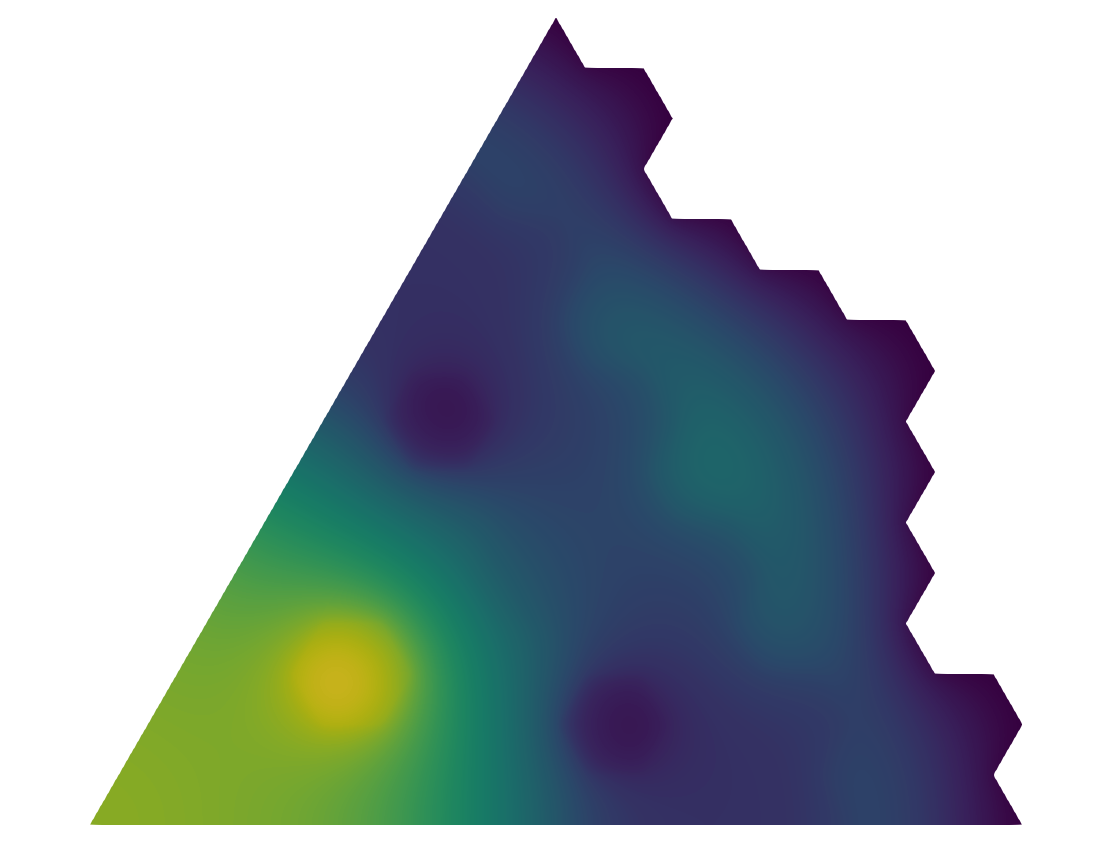
\includegraphics[width=\textwidth]{snr_paraview}
    \caption{Typical Flux Visualization.}
    \label{fig:snr_paraview}
  \end{figure}

  \subsection{Power Iterations}
    \label{sec:power_iterations}
    The FEM is used to solve a fixed source problem for a given source
    distribution $q_g(\vr)$. However, for multigroup problems with scattering, 
    the problem is not a fixed source problem as the source is not known
    explicitly due to interaction between groups. The method of Power Iterations
    allows this multigroup problem to be solved iteratively.

    Recall \eref{eq:multigroup_source} noting the term $q_g(\vr)$. Expanding the
    term $q_g(\vr)$ into its component parts given in \eref{eq:qfiss},
    \eref{eq:qup}, and \eref{eq:qdown}. 
    \begin{equation} \label{eq:multigroup_source_expand}
      -\grad \cdot (D_g(\vr) \grad \phi_g(\vr)) + \Sigma_{r,g}(\vr) \phi_g(\vr) 
        = q_{fiss,g}(\vr) + q_{up,g}(\vr) + q_{down,g}(\vr)
    \end{equation}
    Recall from the definitions of the source components that their calculation
    requires the flux $\phi_g(\vr)$. The source components each require
    different energy groups of the flux distribution to be known. The fission
    component $q_{fiss,g}(\vr)$ requires all groups. The up-scatter component
    $q_{up,g}(\vr)$ requires lower energy groups (i.e. $g' > g$). The
    down-scatter component $q_{down,g}(\vr)$ requires higher energy groups (i.e.
    $g' < g$). Based on these requirements, these source components can be
    calculated based on different power iterations of $\phi_g(\vr)$. This is
    described in Algorithm \ref{algorithm:general}.
    \eref{eq:multigroup_source_expand} is then more explicitly written.
    \begin{equation} \label{eq:multigroup_power_iterations}
      -\grad \cdot (D_g(\vr) \grad \phi_g^{(s)}(\vr)) + \Sigma_{r,g}(\vr)
      \phi_g^{(s)}(\vr) = q_{fiss,g}^{(s-1)}(\vr) + q_{up,g}^{(s-1)}(\vr) +
      q_{down,g}^{(s)}(\vr)
    \end{equation}

  \subsection{Algorithm}
    The algorithm for the solution to the diffusion equation is similar to most
    implementations of the multigroup neutron diffusion method. The algorithm 
    itself is presented in Algorithm \ref{algorithm:general}. The steps unique 
    to the FEM are steps \ref{state:fem_matrix} and \ref{state:fem_vector}. 
    These require the quantities previously derived and form the linear system 
    described by the FEM. 
    
    In step \ref{state:rcm} the matrix is reordered. Mathematically this has no
    effect on the result as the linear system represented is equivalent. This 
    choice to reorder the system is made to improve computational efficiency. 
    Indexing nodes that are physically proximate with proximate indices causes 
    rows in the finite element matrix $\ma$ to be closely coupled to nearby
    rows. In a general unstructured and unordered mesh rows may be coupled to 
    other random rows in the matrix. This step of reordering the matrix $\ma$ 
    seeks to decrease the bandwidth of the matrix and encourage cache hits when
    accessing coupled values in the linear system. The ordering chosen is the
    Reverse Cuthill-McKee (RCM) method and common to sparse linear systems and 
    described in \cite{rcm}.
    
    \begin{algorithm}
      \caption{General Iteration Scheme}
      \label{algorithm:general}
      \begin{algorithmic}[1]
      \State Read mesh from VTK.
      \State Initialize $\phiavg^{(0)}$.
      \State Order the nodes of the mesh into RCM order.
        \label{state:rcm}
      \State Calculate $\Sigma_s$, $\Sigma_t$, and $\nu \Sigma_f$ for each 
        element.
      \State Calculate finite element matrix $\ma_g$ for each group. Store this. 
        \label{state:fem_matrix}
      \While{Power Iteration}
        \State Update the iteration counter. $s=s+1$
        \State Update $q_{fiss,g}$ and $q_{up,g}$ for all gropus from previous 
          data $\phiavg^{(s-1)}$.
        \State Update $\chi$ in each element using previous data.
        \For{$g=1,G$}
          \State Update $q_{down,g}$ from current data $\phiavg^{(s)}$
          \State Calculate total effective source in each element.
          \State Update finite element Vector $\vf_g$ with new source.
            \label{state:fem_vector}
          \State Solve $\ma \vu = \vf$ using an iterative technique (See
            \sref{sec:linear_system_solution}).
          \State Parse $\vu$ for $\phi$ nodal solution.
          \State Calculate element-average $\phiavg$.
        \EndFor
        \State Update $\keff$.
        \State Check convergence.
      \EndWhile
      \end{algorithmic}
    \end{algorithm}
    
    Note that the finite element vector $\vf$ must be updated on each power
    iteration of the solution whereas the matrix $\ma$ is described entirely by 
    geometry and the material cross sections. For this reason, $\ma$ can be 
    generated once at the beginning of the problem and stored for the duration 
    of the calculation.
    \FloatBarrier % make sure the algorithm is in the correct section

  \subsection{Memory and Storage}
    The finite element matrix $\ma$ is large and sparse so a sparse storage and
    sparse solution to the linear system are required. Many sparse matrix 
    implementations have been described and implemented in the past including
    triplet storage, reduced column, and reduced row storage \cite{sparseBLAS}.
    For this application a \twotable method is chosen which was uniquely 
    developed. \twotable storage is not designed to be the most efficient 
    storage method but is chosen for its simplicity and implementation with the 
    FEM. Future work may include a reduced row implementation but there will be
    a trade-off between memory minimization and computational efficiency.
    
    The \twotable method is composed of two separate matrices in memory. An 
    integer index table, \texttt{IDX}, and a double precision value table
    \texttt{VAL}. Each table is dimension $DOF \times D$ where $DOF$ is the
    number of degrees of freedom of the linear system and $D$ is the maximum
    number of nodes that a node shares including itself. This must be determined
    at the beginning of the problem.
    
    \texttt{IDX} is initialized to -1 and \texttt{VAL} is initialized 
    to 0.0 such that an index of -1 corresponds to a null entry in the 
    matrix. \texttt{IDX} is then populated with a modified adjacency graph. 
    Values in \texttt{IDX} indicate the column in which the \texttt{VAL} entry
    occurs. An example unstructured mesh is given in \fref{fig:adjacency_graph}. 
    Then, for node 5, the table \texttt{IDX} may resemble \eref{eq:idx_example}.
    \begin{equation}
      \label{eq:idx_example}
      \texttt{IDX}(5,:) = (8, 200, 48, 96, 5 )
    \end{equation}
    \begin{figure}
      \centering
      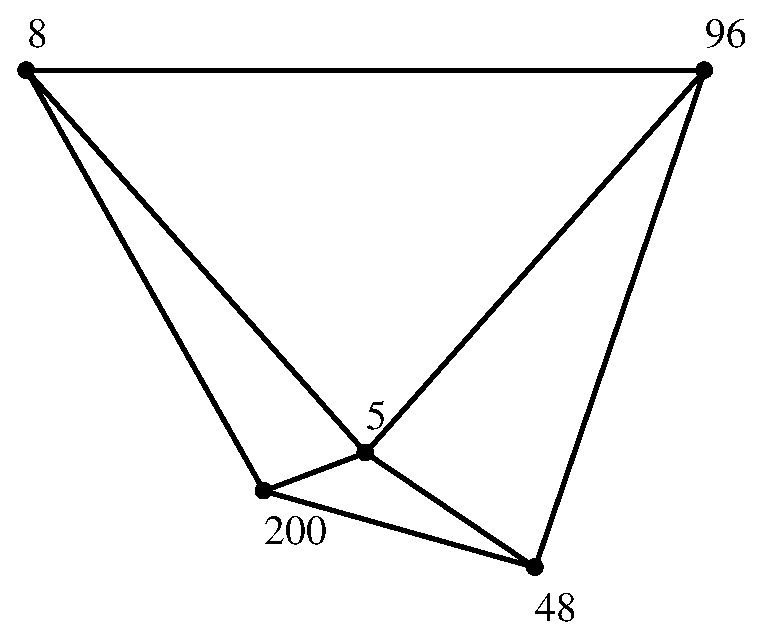
\includegraphics[width=0.5\textwidth]{adjacency_graph}
      \caption{Example Unstructured Mesh.}
      \label{fig:adjacency_graph}
    \end{figure}
    \eref{eq:idx_example} only an example because the order of the nodes in row
    5 is arbitrary. Similarly, a numeric example is provided in 
    \eref{eq:idx_number} (note that the value ``3'' is arbitrary).
    \begin{equation}
      \label{eq:idx_number}
      \left.
      \begin{array}{c}
        \texttt{IDX}(7,3) = 8 \\
        \texttt{VAL}(7,3) = 12.1
      \end{array}
      \right\}
      \implies
      A_{7,8} = 12.1
    \end{equation}
    \eref{eq:idx_number} indicates that the value of matrix $\ma$ in the
    seventh row in the eighth column is 12.1. This will allow for simple row 
    operations and efficient matrix vector multiplication which will be 
    necessary in the solution of the linear system.

  \subsection{Boundary Conditions}
    \label{sec:boundary_conditions}
    Boundary conditions deserve brief consideration. There are many ways to 
    implement boundary conditions and all result in mathematically the same 
    answer. The choices made for this application are presented below. Mirror 
    boundary conditions require $\grad \phi_g(\vr) = 0$ for 
    $\vr \in \partial \Omega$. These are also known as ``natural'' boundary
    conditions because the finite element matrix $\ma$ requires no additional 
    treatment and this condition is natural. In the albedo representation, this
    is equivalent to $\albedo = 0$.
    
    Albedo boundary conditions are treated with an additional contribution to 
    the finite element matrix $\ma$. These contributions represent a line 
    integral in two dimensions and a surface integral in three dimensions. These
    values are found in \eref{eq:matrix_population} and the quantities are 
    expressed in \sref{sec:matrix_quantities} or by quadratures 
    \sref{sec:quadratures}.
    
    Zero-flux boundary conditions require $\phi(\vr) = 0$ for 
    $\vr \in \partial \Omega$. These are treated by removing these entries from
    the finite element matrix $\ma$. Entries are removed by using an index 
    vector. In a natural system (see mirror boundary conditions above) each node
    corresponds to a row/column of the matrix. With entries removed, node number
    and index number may not exactly agree. A vector \texttt{ID} is introduced
    \cite{textbookjohnson}. Nodes with non-zero flux boundary conditions are set
    to a sequential positive integer. Nodes with zero-flux boundary conditions 
    are set to a negative integer (-1) and are omitted in the actual solution of 
    the system. Other strategies have been proposed such as the penalty approach 
    \cite{textbookhughes} and manually forcing the solution of the linear system 
    \cite{textbookli}. This method is chosen because it decreases the degree of 
    freedom of the linear system while encouraging a well conditioned matrix. 
    Now, the degree of freedom of the matrix is equal to the number of nodes 
    with non-zero flux boundary conditions. Alternatively, zero-flux boundary
    conditions can be represented as $\albedo \rightarrow \infty$.
    
  \subsection{Linear System Solution}
    \label{sec:linear_system_solution}
    For a non-singular linear system $\ma \vu = \vf$, where $\ma$ is a square 
    matrix, there exists a unique solution. Many strategies have been proposed 
    to solve this system in an efficient manner. Options are restricted in this
    application because the solution must operate with a sparsely stored linear 
    system and result in no fill-in. This immediately demands an iterative 
    method. The linear system described by the FEM can then be exploited for its 
    unique properties to select a favorable solution method.
    
    The finite element matrix $\ma$ for the problem described in 
    \eref{eq:multigroup_source} is Symmetric Positive Definite (SPD) if the
    multigroup equations are solved one group at a time. Note, the matrix will
    not have this especially useful property if all the groups are solved
    simultaneously. Symmetry condition is straight-forward and is observed in 
    the elemental matrix description \eref{eq:matrix_population}. Briefly,
    $A_{i,j,g,e}=A_{j,i,g,e}$.
    Positive definiteness is a particularly useful condition but is often 
    difficult to prove. $\ma$ is sometimes diagonally dominant for conveniently
    ordered meshes composed certain elements but generally, the matrix is not 
    diagonally dominant. 
    
    A matrix $\ma \in \realnn$ is positive definite if
    \begin{equation} \label{eq:positive_definite}
      \vx^{T} \ma \vx > 0 \qquad \forall \vx \in \realn, \; \vx \ne 0
    \end{equation}
    Following the proof of Theorem 1.9 in \cite{textbookhughes}. Let 
    $\vx = \{x_i\}$ for $i = 1,2,\ldots,N$. Then the vector-matrix and 
    matrix-vector products can be rewritten as summations.
    \begin{equation}
      \vx^{T} \ma \vx = \sum_{i=1}^{N} \sum_{j=1}^{N} x_i A_{ij} x_j
    \end{equation}
    By the definition of $A_{ij}$ in \eref{eq:matrix_population} and 
    \eref{eq:fem_notation}.
    \begin{equation}
      \vx^{T} \ma \vx = 
        \sum_{i=1}^{N} \sum_{j=1}^{N} x_i a(\basis_i,\basis_j) x_j
    \end{equation}
    Noting the property that $a(\cdot,\cdot)$ is a bilinear operator (i.e.
    linear in both arguments) \cite{textbookli}.
    \begin{equation}
      \vx^{T} \ma \vx =
        a \left( \sum_{i=1}^{N} x_i \basis_i, \sum_{j=1}^{N} x_j \basis_j 
        \right)
    \end{equation}
    By construction of the FEM, $w(\vr) = \sum_{i=1}^{N} x_i \basis_i$ where 
    $w(\vr)$ is a piecewise continuous polynomial of arbitrary order.
    \begin{equation}
      \vx^{T} \ma \vx = a \left(w(\vr),w(\vr)\right)
    \end{equation}
    $a(\cdot,\cdot)$ can be shown to form a norm $\|\cdot \|_a$
    \cite{textbookli} satisfying the positive definite condition
    \eref{eq:positive_definite}.
    \begin{equation}
      \vx^{T} \ma \vx > 0 \qquad \forall \vx \in \realn, \; \vx \ne 0
    \end{equation}
    
    A given matrix can be verified as positive definite by one of two methods.
    First, all eigenvalues of the matrix have positive real components. Second, 
    the matrix has a Cholesky decomposition such that $\ma = \ml \ml^*$ where 
    $\ml$ is a lower triangular matrix with positive diagonal entries and 
    $\ml^*$ is the conjugate transpose of the matrix \cite{textbookipsen}. For 
    real valued matrices, the conjugate transpose is equivalent to the 
    conventional transpose. Though this may be useful for debugging or numerical
    analysis purposes, these operations are computationally expensive. Instead,
    this is verified here for the general matrix and not tested on-the-fly.
    
    Conventional methods used to solve a linear system described by an SPD
    matrix include Gauss-Seidel iteration with Successive Over-Relaxation (SOR) 
    and the Conjugate Gradient (CG) Krylov subspace method. SOR needs
    \textit{a priori} knowledge of the optimized over-relaxation factor
    $\omega_{opt}$ for good performanc. In practice, this is performed 
    analytically with contrived solutions or in a modified guess-and-check 
    method. For this application, the CG method is chosen because it requires no 
    \textit{a priori} knowledge and produced a solution to the same tolerance in 
    a comparable wall-time without the need for guess-and-check iterations.
    
    A simple recipe for the CG method is presented in Algorithm 2.4.1
    \cite{Kelley1995IterativeEquations} and its implementation in this 
    application is replicated in Algorithm \ref{algorithm:CG}.
    
    \begin{algorithm}
      \caption{Conjugate Gradient Method}
      \label{algorithm:CG}
      \begin{algorithmic}[1]
        \State $k = 0$
        \State $\vr = \vb - \ma \vx$
        \State $\rho_k = \|\vr\|_2^2$
        \State $k = k + 1$
        \While{$\sqrt{\rho_{k-1}} > \epsilon \|\vb\|_2$}
          \If{$k=1$}
            \State $\vp = \vr$
          \Else
            \State $\beta = \rho_{k-1} / \rho{k-2}$
            \State $\vp = \vr + \beta \vp$
          \EndIf
          \State $\vw = \ma \vp$
          \State $\beta = \rho_{k-1} / \vp^{T} \vw$
          \State $\vx = \vx + \beta \vp$
          \State $\vr = \vr - \beta \vw$
          \State $\rho_k = \| \vr \|_2^2$
          \State $k=k+1$
        \EndWhile
      \end{algorithmic}
    \end{algorithm}
    
    In Algorithm \ref{algorithm:CG}, $\epsilon$ is a tolerance set by the user 
    and the square of the two-norm is most efficiently replaced by the 
    inner-product as in \eref{eq:two_norm_inner}. 
    \begin{equation}
      \label{eq:two_norm_inner}
      \|\vr\|_2^2 = \vr^{T} \vr
    \end{equation}
    It is noted that this method requires minimal storage with only four vectors 
    required ($\vx, \vw, \vp,$ and $\vr$). Additionally, two scalar products 
    are required and a single matrix-vector product which proves to be the most 
    computationally expensive \cite{Kelley1995IterativeEquations}. As most of 
    the computational time of the diffusion solutions is spent in the linear 
    system solution, is is crucial that this process be efficient.
\section{Reference Results}
  This application of the FEM has been compared against reference 
  benchmark problems as well as analytic solutions. Comparison
  against benchmark problems demonstrates an ability to solve problems for
  which this application was intended. Comparison against analytic solutions 
  allows for more detailed error and convergence analysis as not only the system
  $\keff$ but also the exact flux solution are known exactly. 

  Running these comparisons serves as a verification and validation of this
  implementation of the FEM. The strategy used comes from \cite{oberkampf}. The
  first step is ``solution verification.'' Solution verification compares
  computational results to exact analytic results. Verification serves to
  demonstrate that the code itself is solving the correct equations as designed.
  This will be demonstrated with convergence to the analytic answer at the
  expected rate. The second step is ``solution validation.'' Solution validation
  compares computational results to benchmark results which may have been
  calculated computationally via another method or may come from experimental
  data. Validation demonstrates an ability to solve problems for which the
  method was originally intended. The data of the benchmark is not exact, but
  typically the solution has been verified by others previously.
  
  For all reference problems presented, a convergence study is presented. It has 
  been shown that for a bounded second spatial derivative within the problem 
  domain, the FEM derived above is second-order convergent in space
  \cite{textbookli} (Remark 7.13).
  \begin{equation} \label{eq:error_bound}
    \|\ve\|_{\infty} \le c h^2 \| \grad^2 \phi(\vr) \|_{\infty}
  \end{equation}
  Where $\ve$ is the error vector such that $\ve = \phi(\vr) - \phi_{FEM}$ and
  $\phi_{FEM}$ is solution to the finite element system of equations. In
  \eref{eq:error_bound} $h$ is the characteristic mesh size, and $c$ is a 
  constant.  \eref{eq:error_bound} implies that if a characteristic mesh size is 
  halved, the error is quartered. This relationship is useful as a proper 
  implementation of the FEM will converge to the correct answer and do so at the 
  correct rate.
  
  Mesh refinement studies are presented herein. For each refinement, $h$ is 
  halved by introducing new elements and placing new nodes at the midway point
  between existing nodes. Then, let $r$ be the refinement index.
  \begin{equation}
    x = 4 = \frac{x^{(r-1)}}{x^{(r)}}
  \end{equation}
  Such that for some quantity $x$, the error should theoretically decrease by a
  factor of four for each refinement. As these are numerical solutions, the 
  ratio rarely equals exactly four. It is observed that a few refinements are 
  often necessary before the ratio approaches the expected value. This is 
  especially the case when the second derivative is not bounded in problems with 
  heterogeneous materials.
  
  For benchmark problems, only $\keff$ is analyzed and expected to converge
  at the appropriate rate. When assembly powers were available, these are also
  presented graphically. In the graphical power representation, the key is 
  presented in \fref{fig:hex_description}.
  \begin{figure}
    \centering
    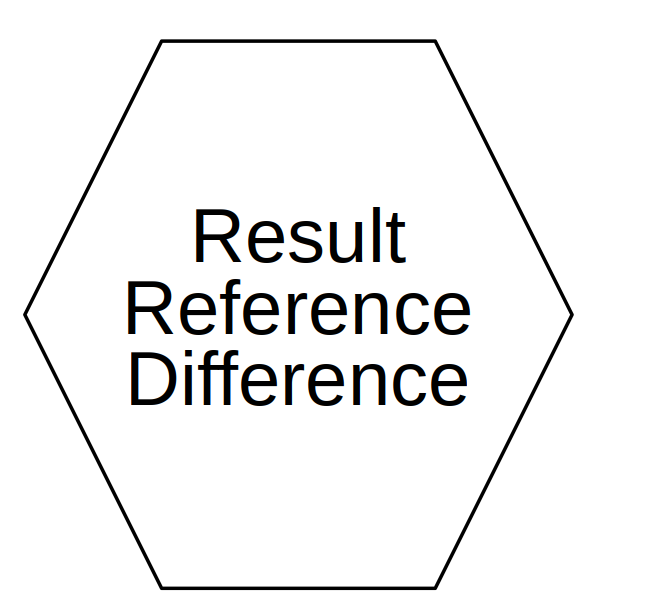
\includegraphics[width=0.25\textwidth]{hex_description}
    \caption{Key for Hexagonal Power Plots.}
    \label{fig:hex_description}
  \end{figure}
  
  For analytic solutions, the error of the function $\phi$ itself can be 
  analyzed because the function is known exactly. The derivations of the exact 
  functions are presented in \apref{ap:analyticSolutions}. For all analytic 
  problems, the Root Mean Squared (RMS) error as in \eref{eq:rms} is calculated
  for the error vector $\ve$ and is presented. The ratio between refinements 
  should assume the expected rate.
  \begin{equation} \label{eq:rms}
    \text{RMS}(\ve) = \sqrt{\frac{1}{N} \sum_{i=1}^{N} e_i}
  \end{equation}
  The maximal norm $\| \cdot \|_{\infty}$ is also presented and the ratio 
  between refinements should assume the expected rate.
  \begin{equation} \label{eq:infnorm}
    \|\ve\|_{\infty} = \max_{i=1,2,\ldots,N} \lvert e_i \rvert
  \end{equation}
  For criticality  problems, $\keff$ is also presented and the ratio between
  refinements should assume the expected rate. $\keff$ error is calculated with
  \eref{eq:keff_err} in units of Percent Mille \units{pcm} from \eref{eq:pcm}.
  \begin{align}
    \label{eq:keff_err}
    \keff \; \text{ error } &= \kref - \keff \\
    \label{eq:pcm}
    x \units{pcm} &= x \; 10^5
  \end{align}

  \subsection{Analytic Solutions}
    As a demonstration of the proper implementation of and solution to the 
    diffusion equation for triangular elements, analytic solutions are 
    derived and then numerically computed. These are one-dimensional,
    two-dimensional, and three-dimensional problems. These problems exercise
    both triangle and wedge elements. For one-dimension problems a rectangular
    domain is used and, the top and bottom edges $y=0$ and $y=L_x$ are mirror
    boundary conditions to reduce the dimension of the problem. 
    To verify there was no error obscured by this process, the results were 
    reproduced for a rotated problem with the left and right edges set to mirror
    boundary conditions as well.
    \subsubsection{One-Dimension, One-Group, Fixed Source}
      \label{sec:1dfixedsrc}
      Arguably the simplest solution to the neutron diffusion equation, this 
      problem  solves a domain $x \in [0,1]$ for a fixed unit source throughout
      the  problem. The exact solution is derived in \sref{sec:deriv_1dfixedsrc}
      and is presented in \eref{eq:analytic_1dfixedsrc}. Results 
      from the convergence study are presented in \tref{tab:1dfixedsrc}.
      \begin{table}
        \caption{One-Dimension, One-Group, Fixed Source Convergence Study 
          Results.}
        \label{tab:1dfixedsrc}
        \begin{center}
          \begin{tabular}{ccccc}
            \toprule
            Refine & RMS & RMS ratio & $\|e\|_{\infty}$ & 
              $\|e\|_{\infty}$ ratio \\
            \midrule
            \csvreader[
              late after line=\\,
              late after last line=\\\bottomrule,]
              {ch02_neutronDiffusion/data/1dfixedsrc.csv}{}
              {\csvcoli & \csvcolii & \csvcoliii & \csvcolviii & \csvcolix}
          \end{tabular}
        \end{center}
      \end{table}
    \subsubsection{One-Dimension, One-Group, Criticality}
      \label{sec:1d1g}
      This problem tests the calculation of the source term and the general 
      iteration implementation in the solution method. This problem solves a 
      fissile material in the domain $x \in [0,100]$.
      The exact solution is derived in \sref{sec:deriv_1d1g} and
      presented in \eref{eq:analytic_1d1g}. Results from
      the convergence study are presented in \tref{tab:1d1g}. The exact value 
      for the effective multiplication factor is $\kref = 1.998028$.
      \begin{table}
        \caption{One-Dimension, One-Group, Criticality Convergence Study
          Results.}
        \label{tab:1d1g}
        \begin{center}
          \begin{tabular}{cccccccccc}
            \toprule
            Refine & $\keff$ & $\keff$ error \units{pcm} & $\keff$ ratio & RMS & 
              RMS ratio  & $\|e\|_{\infty}$ & $\|e\|_{\infty}$ ratio \\
            \midrule
            \csvreader[
              late after line=\\,
              late after last line=\\,]
              {ch02_neutronDiffusion/data/1d1g.csv}{}
              {\csvcoli & \csvcolii & \csvcoliii & \csvcoliv & \csvcolv & 
              \csvcolvi & \csvcolxi & \csvcolxii}
            Ref. & 1.998028 \\
            \bottomrule
          \end{tabular}
        \end{center}
      \end{table}
    \subsubsection{Two-Dimension, One-Group, Criticality}
      This problem tests the ability to solve truly two-dimensional problems.
      The exact solution is derived in \sref{sec:deriv_2d1g} and
       presented in \eref{eq:analytic_2d1g}. Results from
      the convergence study are presented in \tref{tab:2d1g}. The exact value 
      for the effective multiplication factor is $\kref = 1.996060$.
      \begin{table}
        \caption{Two-Dimension, One-Group, Criticality Convergence Study
          Results.}
        \label{tab:2d1g}
        \begin{center}
          \begin{tabular}{cccccccccc}
            \toprule
            Refine & $\keff$ & $\keff$ error \units{pcm} & $\keff$ ratio & RMS & 
              RMS ratio  & $\|e\|_{\infty}$ & $\|e\|_{\infty}$ ratio \\
            \midrule
            \csvreader[
              late after line=\\,
              late after last line=\\,]
              {ch02_neutronDiffusion/data/2d1g.csv}{}
              {\csvcoli & \csvcolii & \csvcoliii & \csvcoliv & \csvcolv & 
              \csvcolvi & \csvcolxi & \csvcolxii}
            Ref. & 1.996060  \\
            \bottomrule
          \end{tabular}
        \end{center}
      \end{table}
    \subsubsection{One-Dimension, Two-Group, Criticality }
      This problem tests the solution of multigroup problems. The results 
      presented are the convergence of $\keff$ and the ratio of relative 
      magnitude of thermal to fast flux $\phi_2/\phi_1$.
      The exact solutions are derived in \sref{sec:deriv_1d2g} and
      the solutions are presented in \eref{eq:twogroupflux1} and
      \eref{eq:twogroupflux2}. Results from the convergence study are presented in 
      \tref{tab:1d2g}. The exact value for the effective multiplication factor 
      is $\kref = 0.892349$ and the exact value for the relative flux ratio
      is $(\phi_2/\phi_1)_{ref} = 0.261324$.
      \begin{table}
        \caption{One-Dimension, Two-Group, Criticality Convergence Study
          Results.}
        \label{tab:1d2g}
        \begin{center}
          \begin{tabular}{ccccccc}
            \toprule
            Refine & $\keff$ & $\keff$ error \units{pcm} & $\keff$ ratio & 
              $\phi_2/\phi_1$ & $\phi_2/\phi_1$ error & $\phi_2/\phi_1$ ratio \\
            \midrule
            \csvreader[
              late after line=\\,
              late after last line=\\,]
              {ch02_neutronDiffusion/data/1d2g.csv}{}
              {\csvcoli & \csvcolii & \csvcoliii & \csvcoliv & \csvcolv & 
              \csvcolvi & \csvcolvii}
            Ref. & 0.892349 &  &  & 0.261324 \\
            \bottomrule
          \end{tabular}
        \end{center}
      \end{table}
    \subsubsection{One-Dimension, One-Group, Two-Region, Criticality}
      This problem tests the mapping of materials to regions within the problem.
      The exact solution is derived in \sref{sec:deriv_2reg} and
      presented in \eref{eq:analytic_2reg}. Results from
      the convergence study are presented in \tref{tab:2reg}. The exact value 
      for the effective multiplication factor is $\kref = 0.962188$.
      \begin{table}
        \caption{One-Dimension, One-Group, Two-Region, Criticality Convergence
          Study Results.}
        \label{tab:2reg}
        \begin{center}
          \begin{tabular}{cccccccccc}
            \toprule
            Refine & $\keff$ & $\keff$ error \units{pcm} & $\keff$ ratio & RMS & 
              RMS ratio  & $\|e\|_{\infty}$ & $\|e\|_{\infty}$ ratio \\
            \midrule
            \csvreader[
              late after line=\\,
              late after last line=\\,]
              {ch02_neutronDiffusion/data/2reg.csv}{}
              {\csvcoli & \csvcolii & \csvcoliii & \csvcoliv & \csvcolv & 
              \csvcolvi & \csvcolxi & \csvcolxii}
            Ref. & 0.962188 \\
            \bottomrule
          \end{tabular}
        \end{center}
      \end{table}
    \subsubsection{Three-Dimension, One-Group, Finite Cylinder}
        This problem is a finite cylinder with zero-flux
        boundary conditions. The cylinder is three-dimensional but the solution
        can be reduced to two dimensions (radial and axial directions). 
        The exact solution is derived in \sref{sec:deriv_finite_cyl} and the
        solution is presented in \eref{eq:analytic_finite_cyl}. Results from the
        convergence study are presented in \tref{tab:finite_cyl}. The exact value
        for the effective multiplication factor is $\kref = 0.996711$.
        \begin{table}
          \caption{Finite Cylinder Convergence Study Results.}
          \label{tab:finite_cyl}
          \begin{center}
            \begin{tabular}{cccccccccc}
              \toprule
              Refine & $\keff$ & $\keff$ error \units{pcm} & $\keff$ ratio & RMS & 
                RMS ratio  & $\|e\|_{\infty}$ & $\|e\|_{\infty}$ ratio \\
              \midrule
              \csvreader[
                late after line=\\,
                late after last line=\\,]
                {ch02_neutronDiffusion/data/finite_cyl.csv}{}
                {\csvcoli & \csvcolii & \csvcoliii & \csvcoliv & \csvcolv & 
                \csvcolvi & \csvcolxi & \csvcolxii}
              Ref. & 0.996711 \\
              \bottomrule
            \end{tabular}
          \end{center}
        \end{table}
  \subsection{Benchmark Solutions}
    The application presented here was designed 
    simulate power reactors. As such, two-dimension problems with similar
    reactor physics phenomena have been examined here. These two-dimension
    problems come from existing benchmarks based on hexagonal geometry. These
    benchmarks represent various energy group structures, geometries, assembly
    sizes,  boundary conditions, as well as other properties. Data used in these
    problems is concisely presented in \apref{ap:benchmarks}. 
    \subsubsection{VVER440}
      Proposed in \cite{chao} and described in \sref{sec:vver440}, this
      benchmark, two-dimensional problem is based on a
      VVER-440 reactor. The VVER-440 is a 
      light-water moderated reactor and operates principally with thermal 
      neutron spectrum. Cross sections are provided for a two-group energy 
      structure.
      
      Power comparison between the most refined mesh and the reference solution 
      are presented graphically in \fref{fig:diffusion_vver440} according to the
      key in \fref{fig:hex_description}. Numerical mesh convergence study for 
      the quantity $\keff$ is presented in \tref{tab:vver440}.
      \begin{figure}
        \centering
        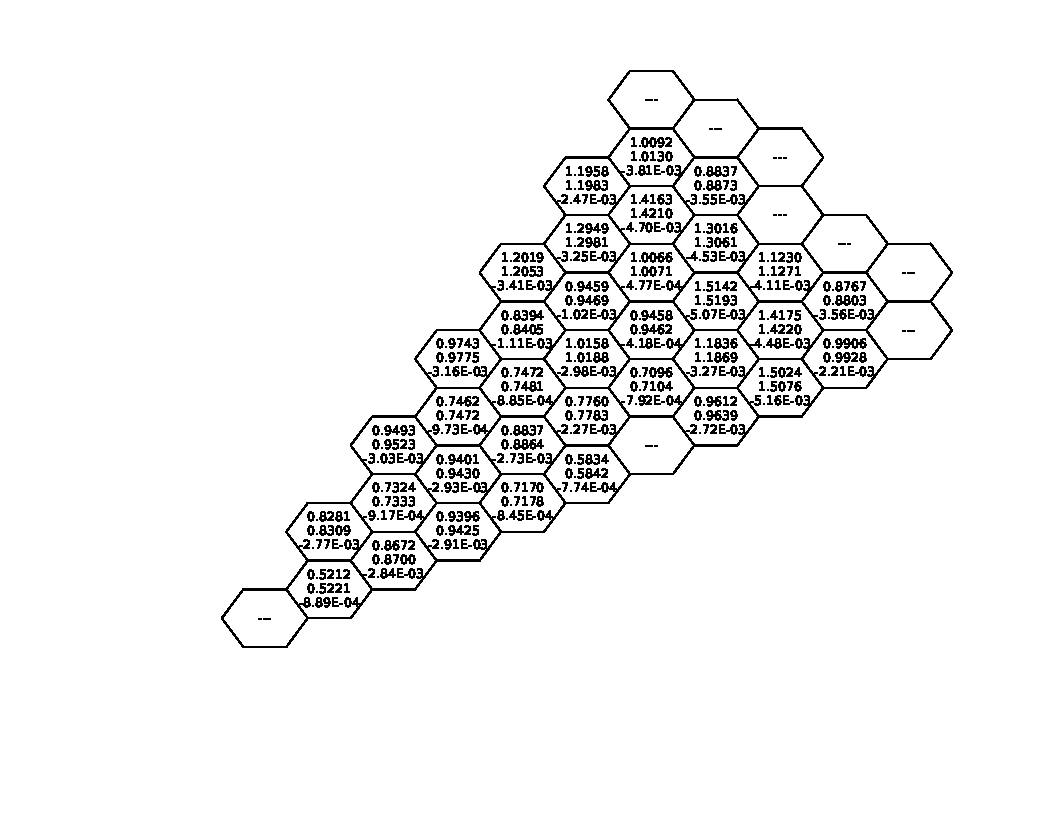
\includegraphics[width=\textwidth]{diffusion_vver440}
        \caption{VVER440 Benchmark Power Comparison for Most Refined Mesh.}
        \label{fig:diffusion_vver440}
      \end{figure}
      \begin{table}
        \begin{center}
          \caption{VVER440 Benchmark Convergence Study.}
          \label{tab:vver440}
          \begin{threeparttable}
            \begin{tabular}{cccc}
              \toprule
              Refine & $\keff$ & $\keff$ error \units{pcm} & $\keff$ ratio \\
              \midrule
              \csvreader[
                late after line=\\,
                late after last line=\\,]
                {ch02_neutronDiffusion/data/vver440.csv}{}
                {\csvcoli & \csvcolvi & \csvcolvii & \csvcolviii}
              Ref.\tnote{$\dagger$}  & 1.009700 \\
              \bottomrule
            \end{tabular}
            \begin{tablenotes}
              \item[$\dagger$] See \cite{chao}.
            \end{tablenotes}
          \end{threeparttable}
        \end{center}
      \end{table}
    \subsubsection{SNR}
      Proposed in \cite{argonneBenchmark} and described in \sref{sec:snr}, this
      benchmark, two-dimensional problem is based on a SNR reactor. The SNR
      is a sodium cooled fast reactor and operates principly with thermal
      neutrons. Cross sections are provided for a four-group energy structure.

      Power comparision between the most refined mesh and numerical solution
      given by DIF3D are presented graphicall in \fref{fig:diffusion_snr}
      according to the key in \fref{fig:hex_description}. Numerical mesh
      convergence study for the quantity $\keff$ is presented in \tref{tab:snr}.
      \begin{figure}
        \centering
        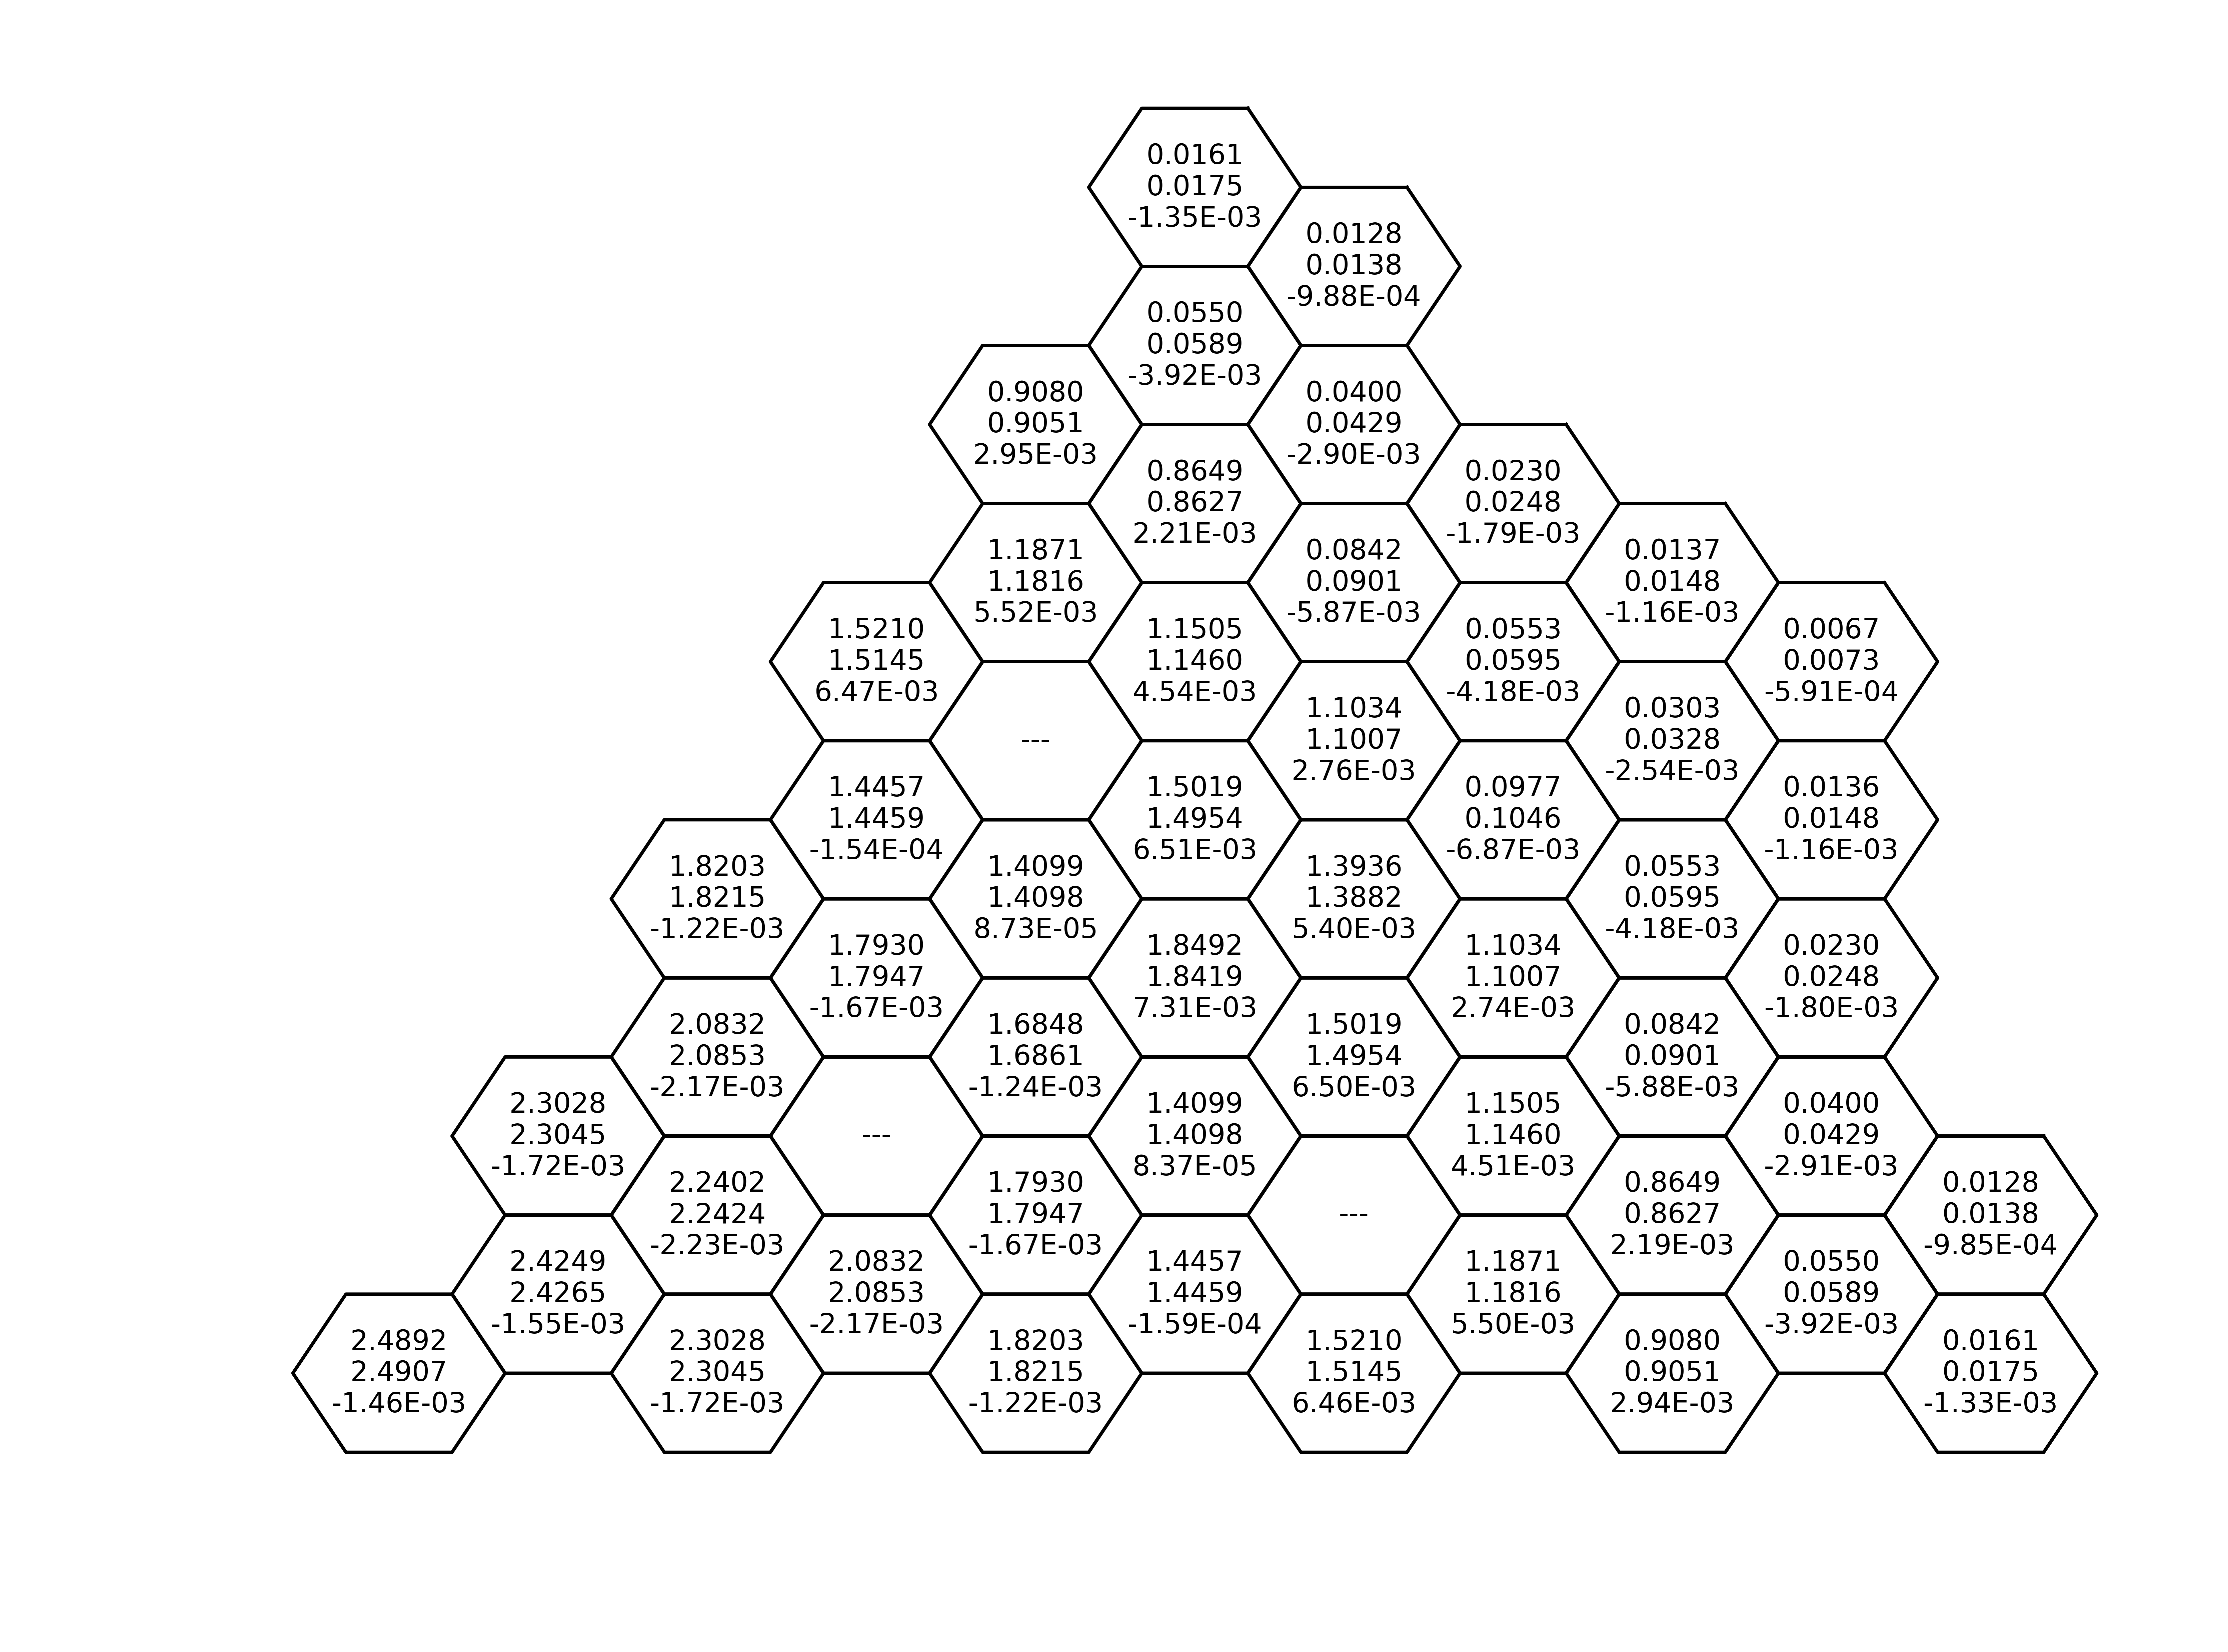
\includegraphics[width=\textwidth]{diffusion_snr}
        \caption{SNR Benchmark Power Comparison for Most Refined Mesh.}
        \label{fig:diffusion_snr}
      \end{figure}
      \begin{table}
        \begin{center}
          \caption{SNR Benchmark Convergence Study.}
          \label{tab:snr}
          \begin{threeparttable}
            \begin{tabular}{cccc}
              \toprule
              Refine & $\keff$ & $\keff$ error \units{pcm} & $\keff$ ratio \\
              \midrule
              \csvreader[
                late after line=\\,
                late after last line=\\,]
                {ch02_neutronDiffusion/data/snr.csv}{}
                {\csvcoli & \csvcolvi & \csvcolvii & \csvcolviii}
              Ref. \tnote{$\dagger$} & 1.124000 \\
              \bottomrule
            \end{tabular}
            \begin{tablenotes}
              \item[$\dagger$] See \cite{argonneBenchmark}.
            \end{tablenotes}
          \end{threeparttable}
        \end{center}
      \end{table}
    \subsubsection{HWR}
      Proposed in \cite{chao} and described in \sref{sec:hwr}, this
      benchmark, two-dimensional problem is based on a large Heavy Water
      Reactor (HWR). This is a heavy water moderated reactor and operates
      principly with thermal neutrons. Cross sections are provided for a
      two-group energy structure.

      Power comparison between the most refined mesh and the reference solution 
      are presented graphically in \fref{fig:diffusion_hwr} according to the
      key in \fref{fig:hex_description}. Numerical mesh convergence study for 
      the quantity $\keff$ is presented in \tref{tab:hwr}.
      \begin{figure}
        \centering
        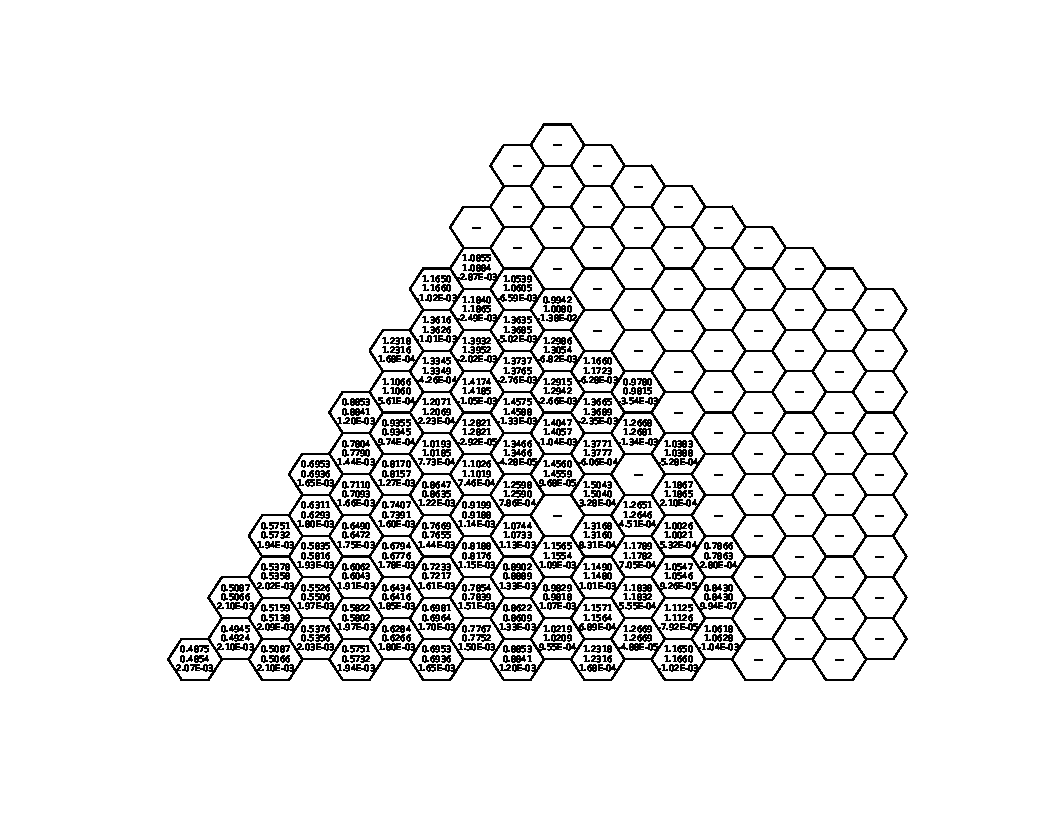
\includegraphics[width=\textwidth]{diffusion_hwr}
        \caption{HWR Benchmark Power Comparison for Most Refined Mesh.}
        \label{fig:diffusion_hwr}
      \end{figure}
      \begin{table}
        \begin{center}
          \caption{HWR Benchmark Convergence Study.}
          \label{tab:hwr}
          \begin{threeparttable}
            \begin{tabular}{cccc}
              \toprule
              Refine & $\keff$ & $\keff$ error \units{pcm} & $\keff$ ratio \\
              \midrule
              \csvreader[
                late after line=\\,
                late after last line=\\,]
                {ch02_neutronDiffusion/data/hwr.csv}{}
                {\csvcoli & \csvcolvi & \csvcolvii & \csvcolviii}
              Ref.\tnote{$\dagger$} & 0.991965  \\
              \bottomrule
            \end{tabular}
            \begin{tablenotes}
              \item[$\dagger$] See \cite{chao}.
            \end{tablenotes}
          \end{threeparttable}
        \end{center}
      \end{table}
    \subsubsection{IAEA}
      Proposed in \cite{chao} and described in \sref{sec:iaea}, this
      reactory-type, two-dimensional problem was originally based on a cartesian
      grid two-dimensional Pressurized Water Reactor (PWR) but was converted to
      hexagonal geometry in \cite{chao}. As it is based on a PWR deisgn, the
      reactor operates principally with thermal spectrum. Cross sections are
      provided for a two-group energy structure.

      The reactor is presented in four scenarios; both with and without
      reflective assemblies as well as with $\albedo = 0.125$ and $\albedo =
      0.5$. Numerical mesh convergence studies are presented for the quantity
      $\keff$ for each case in each of \tref{tab:iaea_nore0125},
      \tref{tab:iaea_nore0500}, \tref{tab:iaea_refl0125}, and
      \tref{tab:iaea_refl0500}.
      % nore0125
      \begin{table}
        \begin{center}
          \caption{IAEA Benchmark Convergence Study. No Reflector. $\albedo = 
            0.125$.}
          \label{tab:iaea_nore0125}
          \begin{threeparttable}
            \begin{tabular}{cccc}
              \toprule
              Refine & $\keff$ & $\keff$ error \units{pcm} & $\keff$ ratio \\
              \midrule
              \csvreader[
                late after line=\\,
                late after last line=\\,]
                {ch02_neutronDiffusion/data/iaea_nore0125.csv}{}
                {\csvcoli & \csvcolvi & \csvcolvii & \csvcolviii}
              Ref. \tnote{$\dagger$} & 0.991378 \\
              \bottomrule
            \end{tabular}
            \begin{tablenotes}
              \item[$\dagger$] See \cite{chao}.
            \end{tablenotes}
          \end{threeparttable}
        \end{center}
      \end{table}
      % nore0500
      \begin{table}
        \begin{center}
          \caption{IAEA Benchmark Convergence Study. No Reflector. $\albedo = 
            0.500$.}
          \label{tab:iaea_nore0500}
          \begin{threeparttable}
            \begin{tabular}{cccc}
              \toprule
              Refine & $\keff$ & $\keff$ error \units{pcm} & $\keff$ ratio \\
              \midrule
              \csvreader[
                late after line=\\,
                late after last line=\\,]
                {ch02_neutronDiffusion/data/iaea_nore0500.csv}{}
                {\csvcoli & \csvcolvi & \csvcolvii & \csvcolviii}
              Ref. \tnote{$\dagger$} & 0.978077 \\
              \bottomrule
            \end{tabular}
            \begin{tablenotes}
              \item[$\dagger$] See \cite{chao}.
            \end{tablenotes}
          \end{threeparttable}
        \end{center}
      \end{table}
      % refl0125
      \begin{table}
        \begin{center}
          \caption{IAEA Benchmark Convergence Study. With Reflector. $\albedo = 
            0.125$.}
          \label{tab:iaea_refl0125}
          \begin{threeparttable}
            \begin{tabular}{cccc}
              \toprule
              Refine & $\keff$ & $\keff$ error \units{pcm} & $\keff$ ratio \\
              \midrule
              \csvreader[
                late after line=\\,
                late after last line=\\,]
                {ch02_neutronDiffusion/data/iaea_refl0125.csv}{}
                {\csvcoli & \csvcolvi & \csvcolvii & \csvcolviii}
              Ref. \tnote{$\dagger$} & 1.006630 \\
              \bottomrule
            \end{tabular}
            \begin{tablenotes}
              \item[$\dagger$] See \cite{chao}.
            \end{tablenotes}
          \end{threeparttable}
        \end{center}
      \end{table}
      % refl0500
      \begin{table}
        \begin{center}
        \caption{IAEA Benchmark Convergence Study. With Reflector. $\albedo = 
          0.500$.}
        \label{tab:iaea_refl0500}
          \begin{threeparttable}
            \begin{tabular}{cccc}
              \toprule
              Refine & $\keff$ & $\keff$ error \units{pcm} & $\keff$ ratio \\
              \midrule
              \csvreader[
                late after line=\\,
                late after last line=\\,]
                {ch02_neutronDiffusion/data/iaea_refl0500.csv}{}
                {\csvcoli & \csvcolvi & \csvcolvii & \csvcolviii}
              Ref. \tnote{$\dagger$} & 1.005507 \\
              \bottomrule
            \end{tabular}
            \begin{tablenotes}
              \item[$\dagger$] See \cite{chao}.
            \end{tablenotes}
          \end{threeparttable}
        \end{center}
      \end{table}
    \subsubsection{MONJU}
      Proposed in \cite{monjuBenchmark} and described in \sref{sec:monju}, this 
      three-dimension, reactory-type problem is based on a Sodium-cooled Fast
      Reactor (SFR) operating principally with fast neutrons. Cross sections are
      provided for a three-group energy structure. However, the fission spectrum
      is not provided and is selcted for benchmark agreement. This assumed
      fission spectrum is presented in \tref{tab:monjuchi}. The rod worth
      measurements appear insensitive to fission spectrum. 

      Reference data can be found in \tref{tab:monjukeff}. Results from the
      finite element application are presented in \tref{tab:monju}. The error
      (difference between reference and calculated results) are presented in
      parenthesis next to the quantities. 

      Rod Worth is presented in units \units{$\Delta$ k} and calculated in
      \eref{eq:rodworth} for $x = \{B,C\}$. Rod Difference is presented in units 
      \units{\%$\Delta$k} where $x \units{\%$\Delta$k} = x \cdot 100$ and is
      calculated in \eref{eq:roddifference} for $x = \{B,C\}$.
      \begin{align}
        \label{eq:rodworth}
        \text{Rod Worth}_x = \frac{k_A - k_x}{k_A k_x} \\
        \label{eq:roddifference}
        \text{Rod Difference}_x = k_A - k_x
      \end{align}
      \begin{table}
        \begin{center}
          \caption{MONJU Benchmark Rod Worth Results. \cite{monjuBenchmark}}
          \label{tab:monju}
          \begin{threeparttable}
            \begin{tabular}{ccll}
              \toprule
              Pattern & $\keff$ & Rod Worth \units{$\Delta k$} & 
                Rod Difference \units{\%$\Delta k$} \\
              \midrule
              A&1.056816&               &            \\
              B&1.031623&0.023 (2.51E-5) \tnote{$\dagger$} &2.52 (-0.07)\\
              C&1.006519&0.047 (1.77E-3)&5.03 (0.04) \\
              \bottomrule
            \end{tabular}
            \begin{tablenotes}
              \item[$\dagger$] Value in parentheses is difference to reference
                value from \cite{monjuBenchmark} as presented in 
                \sref{sec:monju}.
            \end{tablenotes}
          \end{threeparttable}
        \end{center}
      \end{table}
    \subsubsection{KNK}
      Proposed in \cite{takedaBenchmark} and described in \sref{sec:knk}, this
      three-dimension, benchmark problem is based on a SFR and is a model of
      the KNK-II core. Cross sections are provided for a four-group energy
      structure. There are many materials specified in the problem so it also
      aids in testing material mapping in a code. However, the reference data is
      for a transport solution. In this application, the transport cross
      sections are used to solve the neutron diffusion equation. This explains
      some of the numerical differences in the results but general trends are
      reflected. In addition to the comparison to the reference transport
      solution, the neutron diffusion equation is solved with DIF3D and the
      finite element results are comporable to the finite difference solution. 

      Reference data can be found in \tref{tab:knkkeff}. Results from the Finite
      Element neutron diffusion application are presented in \tref{tab:knk}. The
      error (difference between reference and calculated results) are presented
      in parenthesis next to the quantities.

      Rod Worth is presented in units \units{$\Delta$ k} and calculated in
      \eref{eq:rodworth} for $x = \{B,C\}$. Rod Difference is presented in units 
      \units{\%$\Delta$k} where $x \units{\%$\Delta$k} = x \cdot 100$ and is
      calculated in \eref{eq:roddifference} for $x = \{B,C\}$.
      \begin{table}
        \begin{center}
          \caption{KNK Benchmark Rod Worth Results.}
          \label{tab:knk}
          \begin{threeparttable}
            \begin{tabular}{ccll}
              \toprule
              Pattern & $\keff$ & Rod Worth \units{$\Delta k$} & 
                Rod Difference \units{\%$\Delta k$} \\
              \midrule
              A&1.061752&               &            \\
              B&0.942404&0.119 (1.55E-2) \tnote{$\dagger$} &11.93 (0.75)\\
              C&0.829829&0.263 (3.99E-2)&23.19 (1.67)\\
              \bottomrule
            \end{tabular}
            \begin{tablenotes}
              \item[$\dagger$] Value in parentheses is difference to reference
                value from \cite{takedaBenchmark} as presented in 
                \sref{sec:knk}.
            \end{tablenotes}
          \end{threeparttable}
        \end{center}
      \end{table}
